
    In order to study the impact of regional disaster, we augment a standard AS logical connectivity graph~\cite{caida-asgraph} with measurements of the geographic regions in which networks peer.
    We model the Earth as a geodesic globe inscribed in a sphere of the Earth's radius, and map latitude and longitude values to a face on the globe.
    We consider each face of the globe as a `region,' such that a worst-case disaster could destroy all of the physical routing infrastructure within the region.
    We generate the geodesic globe using a standard algorithm~\cite{geodesic}, providing us with 81,000 triangular faces, each with average side length of 100km and area 4700 km$^2$.  
    Finally, we map locations where ASes peer to faces on the globe.
    The same technique could be applied to intradomain connectivity for large networks, but we leave this analysis to future work.    
 
    We develop our peering dataset by borrowing techniques and data from
    the IXP
    Mapping Project~\cite{ixps-mapped}, iPlane~\cite{iplane},
    Aqualab~\cite{sidewalk},
    CAIDA~\cite{caidadata}, and the MaxMind~\cite{maxmind} industrial IP geolocation service.
    For the iPlane and Aqualab data, we derive peering points from raw traceroute files.
    For each pair of IP addresses we observe adjacent in a traceroute, we map the IPs to alias clusters generated by CAIDA's iffinder~\cite{iffinder} and MIDAR~\cite{iffinder, midar} measurements.
    We then map the alias clusters to ASes, and if the ASes are different, we store the two IP addresses as an AS peering.
    Since the majority of stub networks are not geographically widespread, we limited our study to networks which provided transit to at least one AS; thus, we removed any adjacency which included a stub network.
    We map the peering to a geographic location using a combination of DNS-based geolocation and the MaxMind commercial geolocation service.
    For both IP addresses in the adjacency, we do reverse DNS lookups on all IP addresses in their alias clusters. 
    If any of the DNS names match rules from the undns~\cite{undns} or sarang~\cite{sarang} projects, we map the IP address to that location. 
    If multiple of the IP addresses point to different locations, we elect the most common location, or in a tie, choose the location with the least distance from the others.
    If no DNS names are found, we repeat the same process with locations from the MaxMind GeoLite City database, which has better coverage that DNS geolocation, but worse accuracy~\cite{uhlig_ccr_paper}. 
    
    The measurements we gathered from CAIDA, iPlane, and Aqualab allowed us to identify 489,334 router-level AS adjacencies, which we mapped to 14,457 unique latitude, longitude locations (133,686 using DNS, and the remainder using MaxMind).
    We then supplemented these measured adjacencies with 38,994 adjacencies from a ground-truth dataset~\cite{ixps-mapped}, bringing our total to 528,328 adjacencies in 14,571 uniqe latitude, longitude locations. 
    We mapped these adjacencies to 2,900 unique faces of the geodesic globe.   

 
        \subsubsection*{Evaluation of Model}

            To evaluate the representativeness of our data, we investigate the fraction of logically connected ASes for whch we were able to identify geolocated adjecencies, compare our measured adjacencies to a set of ground truth adjacencies, and perform a survey of network operators to validate our data.

            {\bf Representation of Logical Connectivity.} 
            Finite vantage points, policy-based routing, backup links, and limited geolocation capabilities limit our ability to exaustively discover AS adjacencies. 
            Policy-based routing means that traceroutes issued from within a network, or from a network's customer AS, may be able to traverse paths that an issuer from outside the network may not be able to traverse.
            With only finite vantage points limited to a fraction of networks, our measurements may fail to identify many AS-level links.
            Further, backup links between ASes may never be traversed by our traceroute measurements, since backup links are by definition offline unless a failure occurs on a primary link.
            Finally, since geolocation (especially for routers rather than end hosts) is limited, even when we identify an AS-level adjacency we may not be able to geolocate it.
            
            As a first step towards identifying how representative our dataset is, we count how many AS peerings our geolocated adjacencies capture vs those from more exhaustive datasets (note that ground truth data is unavailable).
            \justine{TODO: this.}

            {\bf Ground Truth Adjacencies.}
\begin{figure}[tb]
\centering
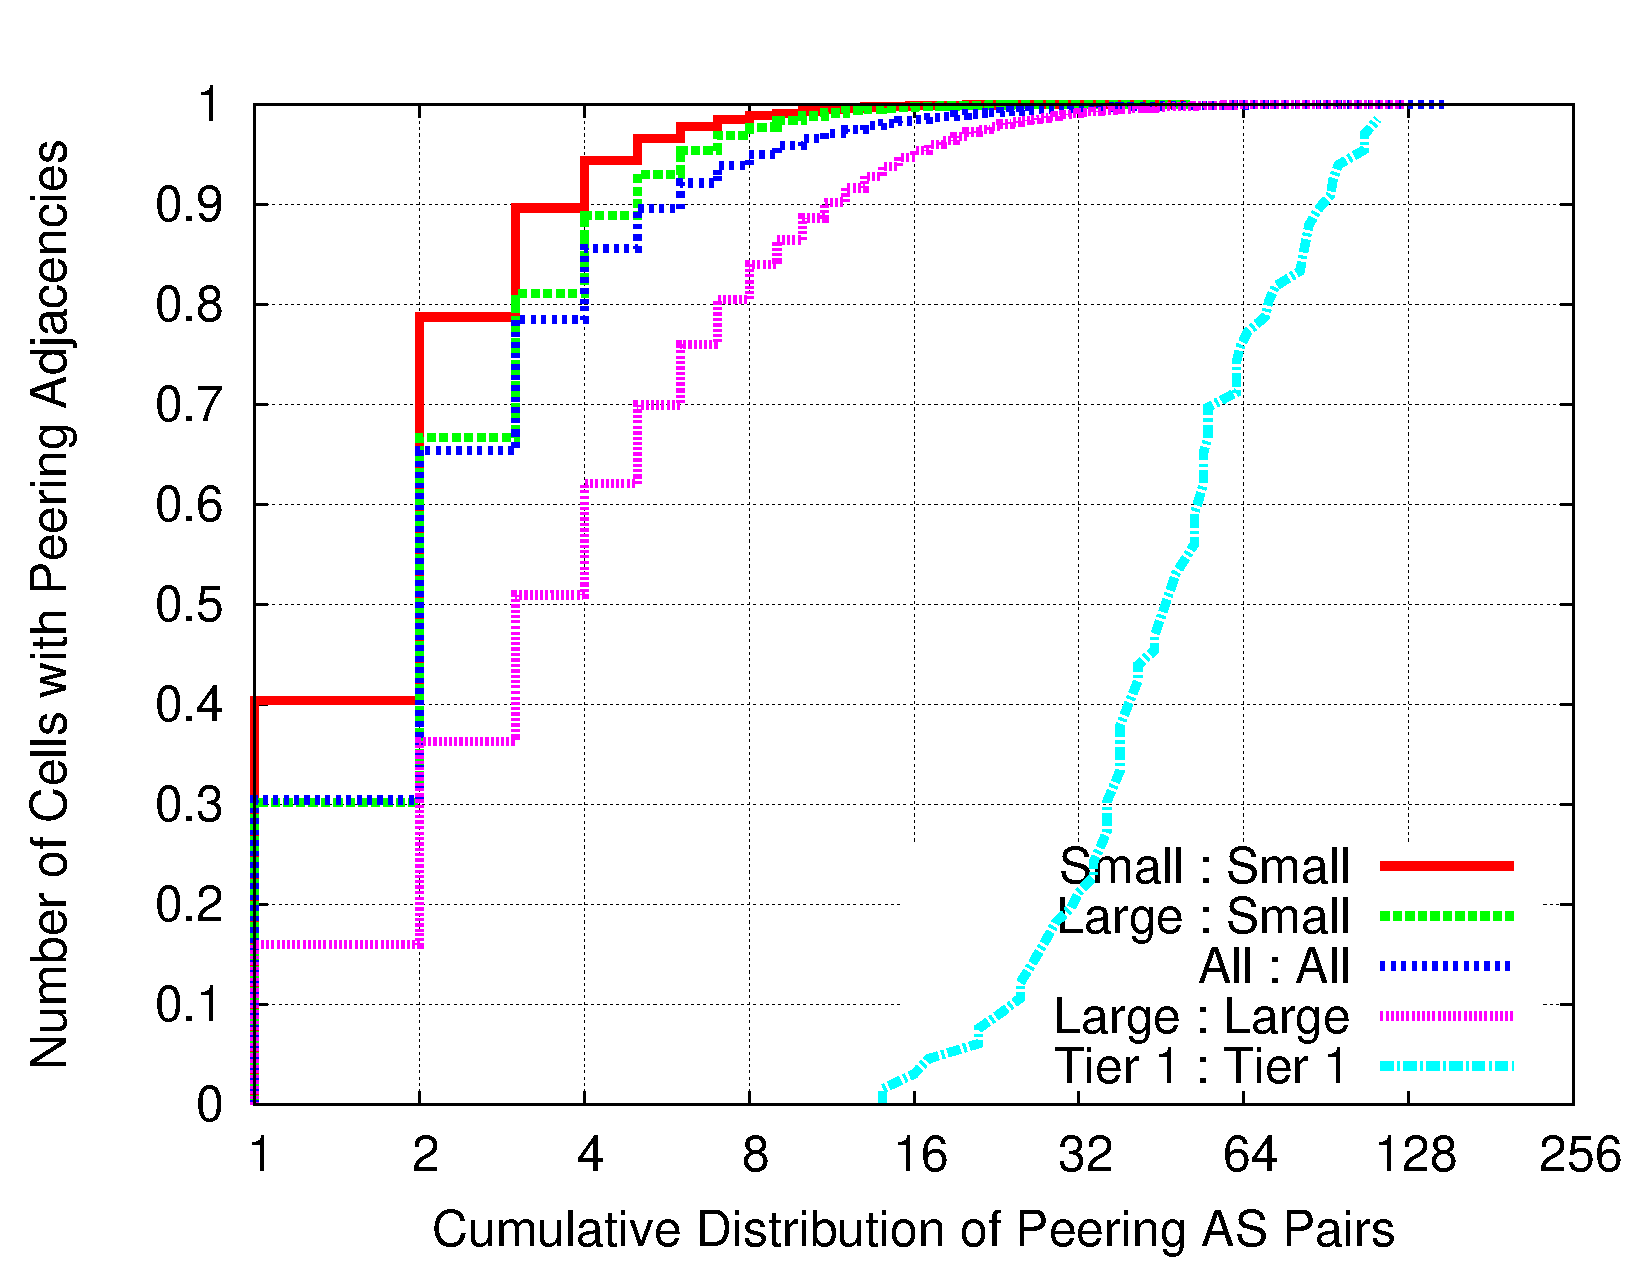
\includegraphics[width=3.25in]{graph_all_match}
\caption[]{\label{fig:closestadjacency} For ground truth peering locations, CCF of distance (kilometers) to closest AS adjacency in our measurement-based dataset. X-axis is in log scale. The average ground truth adjacency is within 100km of a measured adjacency, placing it in either in the same face or a face adjacent to its ground-truth location.} 
\end{figure}
            We next take a set of `ground-truth' adjacencies, peerings with known locations, and compare them to our measured adjacencies. 
           The ground truth adjacencies are borrowed from the IXP Mapping Project~\cite{ixps-mapped}, which manually investigated every public Internet Exchange Point worldwide.
            For each adjacency, we mapped it to the measured adjacency nearest to it on the globe.
            Figure~\cite{fig:closestadjacency} shows the results in CDF form.
            We provide results for comparison to measured adjacencies geolocated using our combined techinique (DNS and Maxmind geolocations both used), DNS geolocation only, MaxMind geolocation only, and strawman geolocation in which all adjacencies are mapped to Greenwich, England.
            \justine{TODO: describe} 




            {\bf Operator Survey.} {\it Due to our poor performance on the previous two metrics, we decided to hold off on our operator survey until we have data we feel confident in sending out for operator validation.}



